

\documentclass[10pt,a4paper]{article}
\usepackage[utf8]{inputenc}
\usepackage[english]{babel}
\usepackage{amsmath}
\usepackage{commath}
\usepackage{mathtools}
\usepackage{amsfonts}
\usepackage{amssymb}
\usepackage{graphicx}
\usepackage{caption}
\usepackage{float}
\usepackage{array}
\usepackage{booktabs}	% for horizontal lines
\usepackage{varwidth}% http://ctan.org/pkg/varwidth
\usepackage{csvsimple} % automatic table generation from csv files
\usepackage{comment}
\usepackage[style=draft, backend=bibtex]{biblatex}
\usepackage[normalem]{ulem}
\useunder{\uline}{\ul}{}


% Macros zum Setzen von Formeln
%-------------------------------

\newcommand{\gradient}[1]{\left(\nabla #1 \right)}
\newcommand{\hesse}[1]{\left(\nabla^2 #1 \right)}
 
% transponiert
\newcommand{\transpose}[1]{#1^\mathrm{T}}
% Exponentialfunktion
\newcommand{\e}{\mathrm{e}}
% Imagin�re Einheit
\newcommand{\I}{\mathrm{I}}
% Einheitsmatrix E
\newcommand{\II}{\vec{E}} 
% Ableitungen
\newcommand{\dd}{\mathop{}\!\mathrm{d}}
\newcommand{\Diff}[2]{\frac{\dd#1}{\dd#2}}
\newcommand{\DiffT}[1]{\Diff{}{t}#1}
\newcommand{\DDiff}[2]{\frac{\dd^2}{\dd#2^2}#1}
\newcommand{\DDiffT}[1]{\DDiff{#1}{t}}
\newcommand{\PartDiff}[2]{\frac{\partial #1}{\partial #2}}
\newcommand{\PartDiffT}[1]{\Diff{#1}{t}}
\newcommand{\PartDDiff}[2]{\frac{\partial^2 #1}{\partial #2^2}}
\newcommand{\PartDDiffT}[1]{\DDiff{#1}{t}}

\newcommand{\lie}[1]{\mathrm{L}_{#1}}
\newcommand{\ad}[1]{\mathrm{ad}_{#1}}

% Betrag und Norm
\newcommand{\abs}[1]{\mleft\vert#1\mright\vert}
\newcommand{\norm}[1]{\mleft\Vert#1\mright\Vert}

% Macro f�r die Abst�nde in Gleichungen mit Nebenbedingungen
\providecommand{\with}{\,, & \qquad}
% Satzzeichen nach Formeln
\providecommand{\FullStop}{\text{~\@.\xspace}}
\providecommand{\Comma}{\text{~,\xspace}}

% Klammern
\providecommand{\of}[1]{\mleft(#1\mright)}
\newcommand{\braces}[1]{\mleft(#1\mright)}
\newcommand{\set}[1]{\mleft\{#1\mright\}}

% Variante f�r \left. und \right\. ohne Abstand
\providecommand{\mleftdot}{\mleft.\kern-\nulldelimiterspace}
\providecommand{\mrightdot}{\mright.\kern-\nulldelimiterspace}

\let\originalleft\left
\let\originalright\right
\renewcommand{\left}{\mleft}
\renewcommand{\right}{\mright}



% Zahlenmengen
\newcommand{\numset}[1]{\mathbbm{#1}}

\newcommand{\eps}{\varepsilon}

% Operatoren
\DeclareMathOperator{\sign}{sgn}
\DeclareMathOperator{\rang}{rang}
\DeclareMathOperator{\Real}{Re}
\DeclareMathOperator{\Imag}{Im}
\DeclareMathOperator{\grad}{grad}
\DeclareMathOperator{\adj}{adj}
\DeclareMathOperator{\Span}{span}
\DeclareMathOperator{\asin}{asin}
\DeclareMathOperator{\acos}{acos}
\DeclareMathOperator{\atan}{atan}
\DeclareMathOperator{\asinh}{asinh}
\DeclareMathOperator{\acosh}{acosh}
\DeclareMathOperator{\atanh}{atanh}

\newcommand{\diag}{\operatorname*{diag}}
\renewcommand{\ker}{\operatorname*{Kern}}
\newcommand{\bild}{\operatorname*{Bild}}
\newcommand{\konst}{\operatorname*{konst.}}
\newcommand{\const}{\operatorname*{const.}}

% Makro f�r Vektoren (unterscheide griechische Buchstaben)
\DeclareRobustCommand{\vec}[1]{ 				
	\ifthenelse{\equal{#1}{\omega} \OR \equal{#1}{\varphi} \OR \equal{#1}{\alpha} \OR \equal{#1}{\beta} \OR \equal{#1}{\chi} \OR \equal{#1}{\delta} \OR \equal{#1}{\varepsilon} \OR \equal{#1}{\phi} \OR \equal{#1}{\epsilon} \OR \equal{#1}{\gamma} \OR \equal{#1}{\eta} \OR \equal{#1}{\iota} \OR \equal{#1}{\kappa} \OR \equal{#1}{\lambda} \OR \equal{#1}{\mu} \OR \equal{#1}{\nu} \OR \equal{#1}{\pi} \OR \equal{#1}{\theta} \OR \equal{#1}{\vartheta} \OR \equal{#1}{\rho} \OR \equal{#1}{\sigma} \OR \equal{#1}{\varsigma} \OR \equal{#1}{\tau} \OR \equal{#1}{\upsilon} \OR \equal{#1}{\xi} \OR \equal{#1}{\psi} \OR \equal{#1}{\zeta}}{
		% F�r griechische Kleinbuchstaben muss boldsymbol verwendet werden (deckt mathbf nicht ab)
		\boldsymbol{#1}
	}{
		% Alle anderen Symbole verwenden mathbf
		\mathbf{#1}
	}
}


%------------------------------
% Macros zur Verwendung im Text
%------------------------------

% Namen
%-------
\providecommand{\Maple}{\textsc{Maple}\xspace}
\providecommand{\Matlab}{\textsc{Matlab}\xspace}
\providecommand{\MatlabSimulink}{\textsc{Matlab/Simulink}\xspace}
\providecommand{\Doxygen}{\textsc{Doxygen}\xspace}

% +++ English
% .\@ is not treated as a full stop (important for the length of the whitespace
% afterwards. \@. is always treated as a full stop.)
\providecommand{\ie}{i.\,e.\@\xspace} 
\providecommand{\eg}{e.\,g.\@\xspace}
\providecommand{\cf}{cf.\@\xspace}

% +++ German
\providecommand{\zB}{z.\,B.\@\xspace}
\providecommand{\ZB}{Z.\,B.\@\xspace}
\providecommand{\bzw}{bzw.\@\xspace}
\providecommand{\bspw}{bspw.\@\xspace}
\AtEndOfClass{\renewcommand{\dh}{d.\,h.\@\xspace}}
\providecommand{\Dh}{D.\,h.\@\xspace}
\providecommand{\ua}{u.\,a.\@\xspace}
\providecommand{\sog}{sog.\@\xspace}
\providecommand{\usw}{usw.\@\xspace}
\providecommand{\etc}{etc.\@\xspace}
\providecommand{\ggf}{ggf.\@\xspace}
\providecommand{\ca}{ca.\@\xspace}
\providecommand{\uU}{u.\,U.\@\xspace}
\providecommand{\vgl}{vgl.\@\xspace}

% f�r W�rter mit Bindestrich. (Setzt einen Bindestrich, an dem nicht getrennt
% werden darf, l�sst aber die Trennung im folgenden Wort zu.)
\providecommand{\hypII}[2]{#1\nobreakdash-\hspace{0pt}#2}
\providecommand{\x}[1]{\hypII{$x$}{#1}}
\providecommand{\y}[1]{\hypII{$y$}{#1}}
\providecommand{\z}[1]{\hypII{$z$}{#1}}

%--- Zeilenhoehe in Tabellen -------------------------------------------------
% Mit dem Befehl \TabEqn kann eine Formel in einer Tabelle gesetzt werden
% (einfach nur die Formel in die Tabelle eingeben bringt die vertikale
% Ausrichtung irgendwie durcheinander)
% \ExtraTabEqnSpace ist der Platz, der oben und unter einer Formel eingef�gt
% wird
\AtEndOfClass{
\newcommand{\ExtraTabEqnSpace}{1ex}
\makeatletter
\newcommand*{\TabEqn}[1]{%
\begingroup
	\setbox\@tempboxa=\hbox{%
	#1%
	}%
	% Hinzufuegung von 1ex zu Hoehe (\ht)
	% und Tiefe (\dp) der Box.
	% Umweg ueber \dimen@ erforderlich,
	% da man \ht, und \dp nur etwas zuweisen,
	% aber nichts hinzufuegen kann.
	\setlength{\dimen@}{\ht\@tempboxa}%
	\addtolength{\dimen@}{\ExtraTabEqnSpace}%
	\setlength{\ht\@tempboxa}{\dimen@}%
	\setlength{\dimen@}{\dp\@tempboxa}%
	\addtolength{\dimen@}{\ExtraTabEqnSpace}%
	\setlength{\dp\@tempboxa}{\dimen@}%
	\usebox\@tempboxa
\endgroup
}
\makeatother
}

\newcommand\mycircle{\@currsize\tikz[baseline=(n.210),inner sep=0pt]%
  \node[line width=0.1em, circle,minimum size=0.7\baselineskip,draw](n){};%
  }
%\myfillcircle[zuf�llender Winkel in Grad]
\newcommand\myfillcircle[1][360]{%
  \@currsize\tikz[baseline=(n.210),inner sep=0pt]%
    \fill(0,0)%
      node[line width=0.1em, circle,minimum size=0.7\baselineskip,draw](n){}%
      --+(0,0.35\baselineskip)%
      arc[start angle=90,end angle=90+#1, radius=0.35\baselineskip];%
}


\addbibresource{../bibliography.bib}

\title{Chapter 3 - Solution Approach DRAFT}
\author{Weber Jakob}

\begin{document}
	\maketitle
	
	\tableofcontents
	%%%%%%%%%%%%%%%%%%%%%%%%%%%%%%%%%%%%%%%%%%%%%%%%%%%%%%%%%%%%%%%%%%%%%%%%%%%%%%%%%%%%%%%%%%%%%%%%%%%%%%%%%%%%%%%%%
	%%%%%%%%%%%%%%%%%%%%%%%%%%%%%%%%%%%%%%%%%%%%%%%%%%%%%%%%%%%%%%%%%%%%%%%%%%%%%%%%%%%%%%%%%%%%%%%%%%%%%%%%%%%%%%%%%
	\section{Introduction}
	
	We are now going to use the theory defined in Chapter 2 to estimate smooth, constraint functions. An overview of the different problems is given in Table \ref{tab:problem_overview}. At first, we are using B-splines as basis functions for the estimation of the one dimensional, unknown function $y = f(x)$ for some data $\{x^{(i)}, y^{(i)}\}$ for $i = 1, \dots, n$.  Next, we use the concept of P-splines introduced by Eilers and Marx in \cite{eilers1996flexible} to estimate smooth, one dimensional functions. Finally, we are going to incorporate a priori knowledge into the fitting process using the approach given by Hofner and apply it to one- and two-dimensional functions. \cite{hofner2011monotonicity} 

	\begin{table}[H]
	\centering
	\begin{tabular}{|lll|}
		\hline
		\textbf{Problem}                   & \textbf{Solution Approach}           & \textbf{Algorithm}  \\ \hline \toprule
		1d Function Estimation             & B-Splines                            & LS                  \\ \hline
		1d Smooth Function Estimation      & P-Splines                            & PLS                 \\ \hline
		1d Constraint Function Estimation  & P-Splines + Constraint Penalty       & PIRLS 			    \\ \hline 
		n-d Constraint Function Estimation & P+TP-Splines + Constraint Penalty & PIRLS 			    \\ \hline \bottomrule
	\end{tabular}
	\caption{Problem overview}
	\label{tab:problem_overview}
	\end{table}

	The a priori knowledge can be incorporated using different types of constraints. The possible constraints are listed in Table \ref{tab:constraint_overview}.
	
	\begin{table}[h]
	\centering
	\begin{tabular}{|lll|}
		\hline
		\textbf{Constraint}& \textbf{Description}                         & \textbf{Math. Description}\\ \hline \toprule
		Monotonicity       & Functions is either increasing or decreasing.& $\lvert f'(x) \rvert \ge 0$ 	\\ \hline
		Curvature          & Function is either convex or concave.        & $\lvert f''(x) \rvert \ge 0$ 	\\ \hline
		Unimodality        & Function has a mode/peak.                    & $m = \arg \max_{x} f(x)$ 				\\ 
						   &	   										  & $f'(x) \ge 0 \quad \text{if} \ x < m$  \\ 
						   &  											  & $f'(x) \le 0 \quad \text{if} \ x > m$  \\ \hline
		Boundedness        & Function is bounded by the value M.          & $\lvert f(x)\rvert \le M$ 		\\ \hline
		Jamming            & Function is jammed by the value M.           & $f(x^{(M)}) \approx y^{(M)}$	\\ \hline \bottomrule
	\end{tabular}
	\caption{Overview of the possible constraints}
	\label{tab:constraint_overview}
	\end{table}
		
	To test the algorithm and the incorporation of a priori knowledge, we use 200 noisy samples, see Figure \ref{fig:test_func}, from the one dimensonal function given in (\ref{eq:test_func}) and the monotonicity constraint. 
	
	\begin{align}\label{eq:test_func}
	f(x) = 3\sin(3\pi x) + 17x + 3
	\end{align}
	
	The function is purposely chosen such that the samples violate the constraint for some $x$. 
	
	\begin{figure}[H]
		\centering
		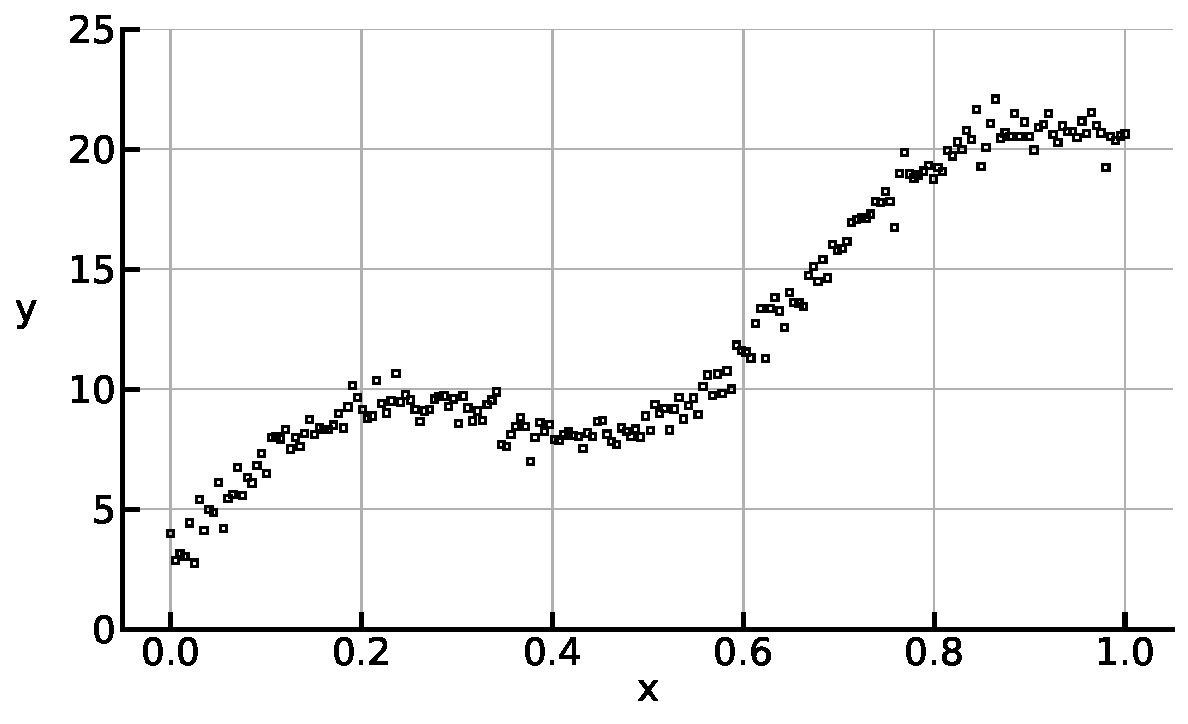
\includegraphics[width=\columnwidth]{../thesisplots/test_func.pdf}
		\caption{Noisy samples from Function \ref{fig:test_func}}
		\label{fig:test_func}
	\end{figure}

	%%%%%%%%%%%%%%%%%%%%%%%%%%%%%%%%%%%%%%%%%%%%%%%%%%%%%%%%%%%%%%%%%%%%%%%%%%%%%%%%%%%%%%%%%%%%%%%%%%%%%%%%%%%%%%%%%
	\section{Function Estimation}
	
	\subsection{1d Function Estimation} \label{1D}
 	 
 	The goal is to model given data
 	
 	\begin{align} \label{eq:data}
 		\{x^{(i)}, y^{(i)}\}, \quad i = 1, \dots, n 
 	\end{align}
 	
	using B-splines as basis functions. Therefore we want to estimate the unknown function $y = f(x)$ which can be represented as a linear combination of $k$ B-spline basis functions $x_k$ as
	
	\begin{align} \label{eq:basis_function_approach}
		y = f(x) = \sum_{j=1}^k \beta_k x_k(x) = \vec{X} \vec{\beta},
	\end{align}
	
	where $\vec{X} \in \mathbb{R}^{n\times k}$ is the B-spline basis matrix and $\vec{\beta} \in \mathbb{R}^k$ are the coefficients to be estimated. 
	
 	The least squares objective function to be minimized using the complete data is then given by
	
	\begin{align} \label{eq:OF_1}
		Q_1(\vec{y}, \vec{\beta}) = \lVert \vec{y} - f(\vec{x}) \rVert^2 = \lVert \vec{y} - \vec{X}\vec{\beta} \rVert^2 
	\end{align}	
	
	The coefficients are determined by minimizing the objective function given in (\ref{eq:OF_1}) with respect to $\vec{\beta}$, i.e.
	
	\begin{align}\label{eq:optimization_problem_1}
		\vec{\hat \beta}_{LS} = \arg \min_{\vec{\beta}} Q_1(\vec{y}, \vec{\beta}).
	\end{align}
	
	Using the least squares algorithm LS, this yields 
	
	\begin{align} \label{eq:LS_coef}
		\vec{\hat \beta}_{LS}= (\transpose{\vec{X}} \vec{X})^{-1} \transpose{\vec{X}} \vec{y}.
	\end{align} 
	
	
	Figure \ref{fig:smooth_bf} shows a B-spline model using $k=10$ splines on an equidistant grid approximating the noisy data as well as the individual B-spline basis functions multiplied with the corresponding, estimated coefficients $\vec{\hat \beta}_{LS}$.
	
	\begin{figure}[H]
		\centering
		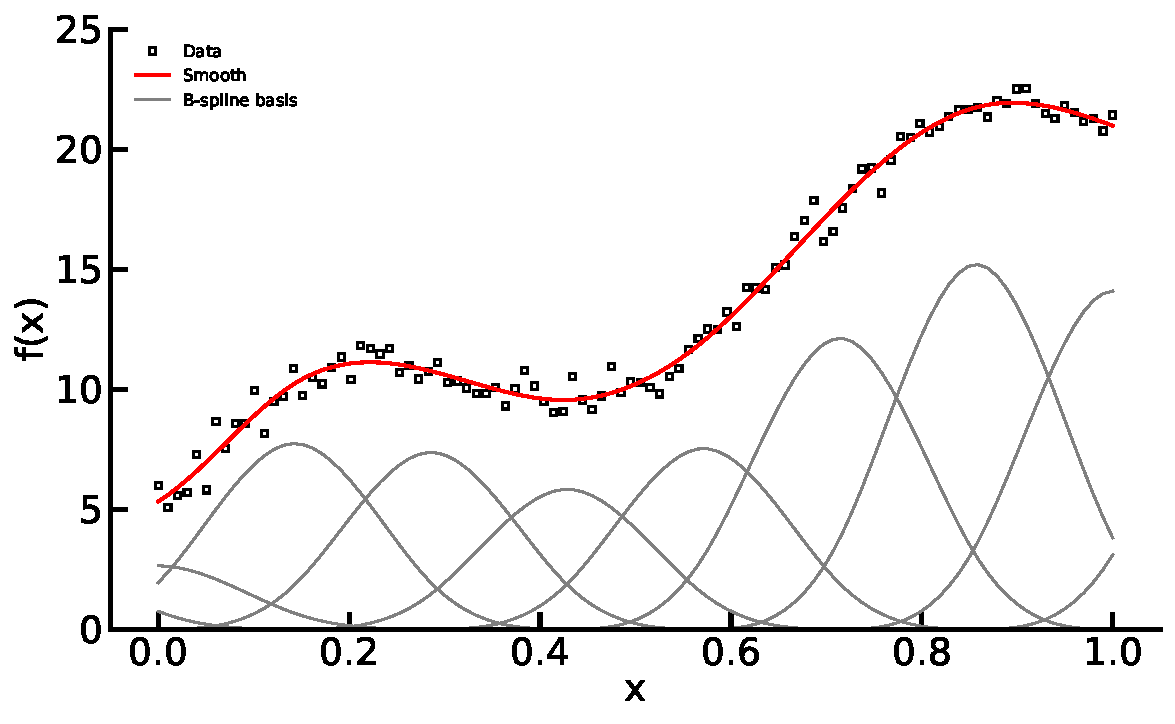
\includegraphics[width=\columnwidth]{../thesisplots/smooth_bf.pdf}
		\caption{Approximation of noisy data by B-splines without constraints}
		\label{fig:smooth_bf}
    \end{figure}
	
	
	The number of splines $k$ has a strong influence on the amount of smoothing. A small number $k$ leads to a very smooth estimate, but a large data error. On the other hand, when the number of splines is relatively large, the data error is very small but the smoothness of the estimate is poor. This behavior is an example of the bias-variance dilemma and depicted in Figure \ref{fig:smooth_bf_large}. \cite{sammut2011}


	\begin{figure}[H]
	\centering
	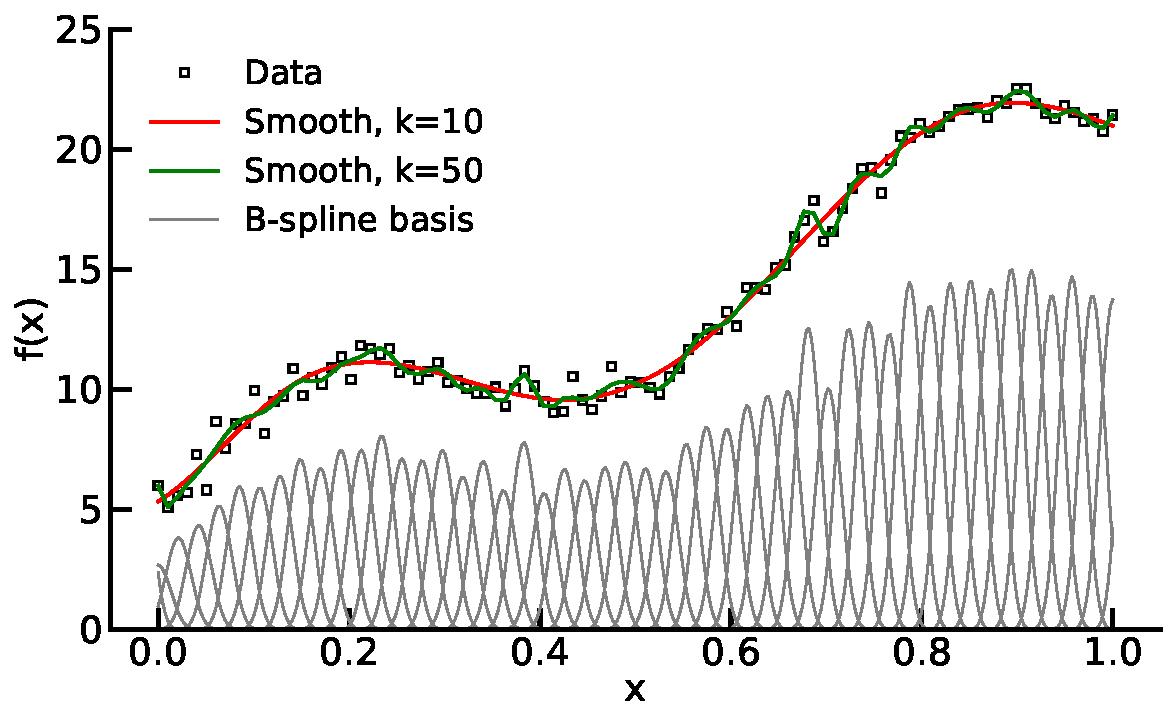
\includegraphics[width=\linewidth]{../thesisplots/smooth_wiggly_bf.pdf}
	\caption{Approximation of noisy data by 10 and 50 B-splines without constraints}
	\label{fig:smooth_bf_large}
	\end{figure}


	%%%%%%%%%%%%%%%%%%%%%%%%%%%%%%%%%%%%%%%%%%%%%%%%%%%%%%%%%%%%%%%%%%%%%%%%%%%%%%%%%%%%%%%%%%%%%%%%%%%%%%%%%%%%%%%%%
	\subsection{1d Smooth Function Estimation} \label{1D_smooth}

	To overcome this problem, the second derivative of the estimated function $f(x)$, i.e. $f''(x) = \sum_{j=1}^k \beta_k x_k''(x)$, has to be penalized to realize a smoother estimate. Eilers and Marx have introduced the so-called P-splines. \cite{eilers1996flexible} Therefore, the objective function (\ref{eq:OF_1}) is extended by an additional term considering the smoothness, 
	
	\begin{align}\label{eq:OF_2}
		Q_2(\vec{y}, \vec{\beta}) = Q_1(\vec{y}, \vec{\beta}) + \lambda_s \mathcal{J}_s(\vec{\beta}; d) = \lVert \vec{y} - \vec{X} \vec{\beta} \rVert^2 + \lambda_s \transpose{\vec{\beta}} \transpose{\vec{D}}_d \vec{D}_d \vec{\beta}, 
	\end{align}
	
	with the smoothing parameter $\lambda_s$ and an appropriate mapping matrix $\vec{D}_d$ capturing the second derivative, which itself is a measure for function wiggliness. Here, an approximation of the second derivative can be performed by the squared finite difference of order $d$ of adjacent coefficients using the matrix form of the difference operator of order $d$. 
	
	The difference operator  $\Delta^d$ of order $d$ for equidistant knot placement of B-splines is defined by
	
	\begin{align*}
		\Delta^1 \beta_j &= \beta_j - \beta_{j-1} \\
		\Delta^2 \beta_j &= \Delta^1(\Delta^1 \beta_j) = \beta_j - 2\beta_{j-1} + \beta_{j-2} \\ 
	  	\vdots \\ 
	  	\Delta^d \beta_j &= \Delta^1(...(\Delta^1 \beta_j))
	\end{align*}
	
	and in matrix notation for order $d=1$
	
	$$\vec{D}_1 = 
			\begin{pmatrix} 
					-1& 1&       &        &   \\  
					  &-1& 1     &        &   \\  
					  &  &\ddots & \ddots &   \\ 
					  &  &       & -1     & 1 
			\end{pmatrix} \in \mathbb R^{k-1\times k}$$
	
	and order $d=2$
	
	$$\vec{D}_2 = 
			\begin{pmatrix} 
				1& -2& 1& &    \\  
				 & 1 & -2 & 1& \\ 
				 &  & \ddots & \ddots  & \ddots \\ 
				 & & & 1 & -2 & 1 
			\end{pmatrix} \in \mathbb R^{k-2\times k}.$$
	
	For non-equidistant knot placement, the difference operator $\Delta^d$ needs to include some kind of weighting determining the influence of the individual splines. A possible approach can be found in \cite{ferziger2008numerische}.
	
	By minimizing the objective function (\ref{eq:OF_2}), i.e.
	
	\begin{align}\label{eq:optimization_problem_2}
		\vec{\hat \beta}_{PLS} = \arg \min_{\vec{\beta}} Q_2(\vec{y}, \vec{\beta}),
	\end{align}
	
	using the penalized least squares algorithm PLS, the penalized least squares coefficients are given by
	
	\begin{align} \label{eq:PLS_coef}
		\vec{\hat \beta}_{PLS}= (\transpose{\vec{X}} \vec{X} + \lambda_s \transpose{\vec{D}}_d \vec{D}_d)^{-1} \transpose{\vec{X}} \vec{y}.
	\end{align} 
	
	The smoothing parameter $\lambda_s$ plays a critical role and can be optimized using the information criteria specified in Chapter Model Selection Criteria, e.g. AIC and BIC, or by using cross-validation techniques. \cite{fahrmeir2013regression}
	For small values $\lambda_s \rightarrow 0$, the penalized least squares estimate $\vec{\hat{\beta}}_{PLS}$ approaches the least squares estimate $\vec{\hat{\beta}}_{LS}$, while for large values $\lambda_s \gg 0$, the fitted function shows the behavior of a polynomial with $d-1$ degrees of freedom. For example, using $d=2$ and a large smoothing parameter $\lambda_s$ is leading to a linear function, while using $d=1$ would lead to a constant function. \cite{fahrmeir2013regression}
	
	Figure \ref{fig:pspline} shows the behavior of P-splines using $k=50$ splines for several values of the smoothing parameter $\lambda_s = \{10^{-2}, 10^{2},10^{5},10^{6}\}$ and a smoothness penalty of order $d=2$.  As the value of $\lambda_s$ gets larger, the fitted curve becomes more smooth and thus the $2^{nd}$ derivative becomes smaller. For very large values of $\lambda$, the estimate approaches a straight line.
	
	\begin{figure}[H]
		\centering
		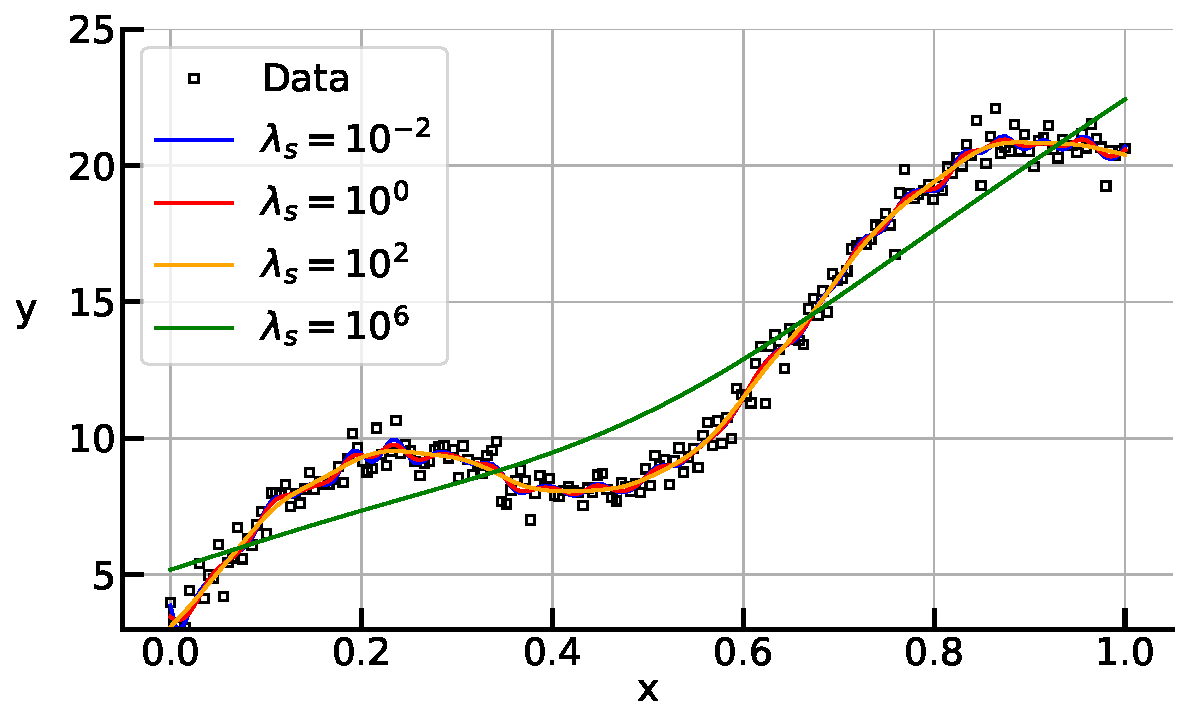
\includegraphics[width=\linewidth]{../thesisplots/p_splines.pdf}
		\caption{Smooth function estimation for different $\lambda_s$}
		\label{fig:pspline}
	\end{figure}

	%%%%%%%%%%%%%%%%%%%%%%%%%%%%%%%%%%%%%%%%%%%%%%%%%%%%%%%%%%%%%%%%%%%%%%%%%%%%%%%%%%%%%%%%%%%%%%%%%%%%%%%%%%%%%%%%%
	\subsection{1d Constraint Function Estimation}
	
	A priori knowledge can now be systematically incorporated by the extension of the objective function (\ref{eq:OF_2}) using an additional term representing the user-defined constraint. Note that this approach incorporates the a priori knowledge as soft constraints. Therefore, no guarantee can be given that the fit holds the constraint for every possible input. The constraint penalized least-squares objective function is given by
	
	\begin{align}\label{eq:OF_3}
		Q_3(\vec{y}, \vec{\beta}) = Q_1(\vec{y}, \vec{\beta}) + \lambda_s \mathcal{J}_s(\vec{\beta}; d) + \lambda_c \mathcal{J}_c(\vec{\beta}; c)
	\end{align}
	
	with the corresponding constraint parameter $\lambda_c$, which determines the influence of the constraint. Note that the parameter $\lambda_c$ has to be set quite large, i.e. $\lambda_c > 10^4$, compared to $\lambda_s$ to enforce the user-defined constraint. 
	
	Constraints for monotonicity, curvature, unimodality and boundedness can be modeled as 
	
	\begin{align} \label{eq:mapping_matrix}
		\mathcal{J}_c(\vec{\beta}; c) = \transpose{\vec{\beta}} \transpose{\vec{D}}_c \vec{V} \vec{D}_c  \vec{\beta}
	\end{align}

	with the mapping matrix $\vec{D}_c$ and the diagonal weighting matrix $\vec{V} \coloneqq \vec{V}(\vec{\beta}; c)$ capturing if the constraint $c$ is active or inactive. These matrices will further be defined in Chapter \ref{sec:user-defined-constraints}.
	
	The constraint of jamming the fit by some critical points can be incorporated using the weighted least squares approach and large weights for the critical points. \cite{strutz2016data}
	
	By minimizing the objective function (\ref{eq:OF_3}), i.e.
	
	\begin{align}\label{eq:optimization_problem_3}
		\vec{\hat \beta}_{PLS, c} = \arg \min_{\vec{\beta}} Q_3(\vec{y}, \vec{\beta}),
	\end{align}
	
	the constraint penalized least-squares estimate can be given as
	
	\begin{align} \label{eq:PLS,c_coef}
		\vec{\hat \beta}_{PLS, c} = (\transpose{\vec{X}} \vec{X} + \lambda_s \transpose{\vec{D}}_d \vec{D}_d + \lambda_c \transpose{\vec{D}}_c \vec{V} \vec{D}_c)^{-1} \transpose{\vec{X}} \vec{y}.
	\end{align}	
 
 	Note, (\ref{eq:PLS,c_coef}) is a nonlinear equation because the matrix $\vec{V}$ depends on $\vec{\beta}$. Thus, it has to be solved iteratively. The algorithm is shown in Figure \ref{fig:pirls}. 
 	
 	\begin{figure}[H]
 		\centering
 		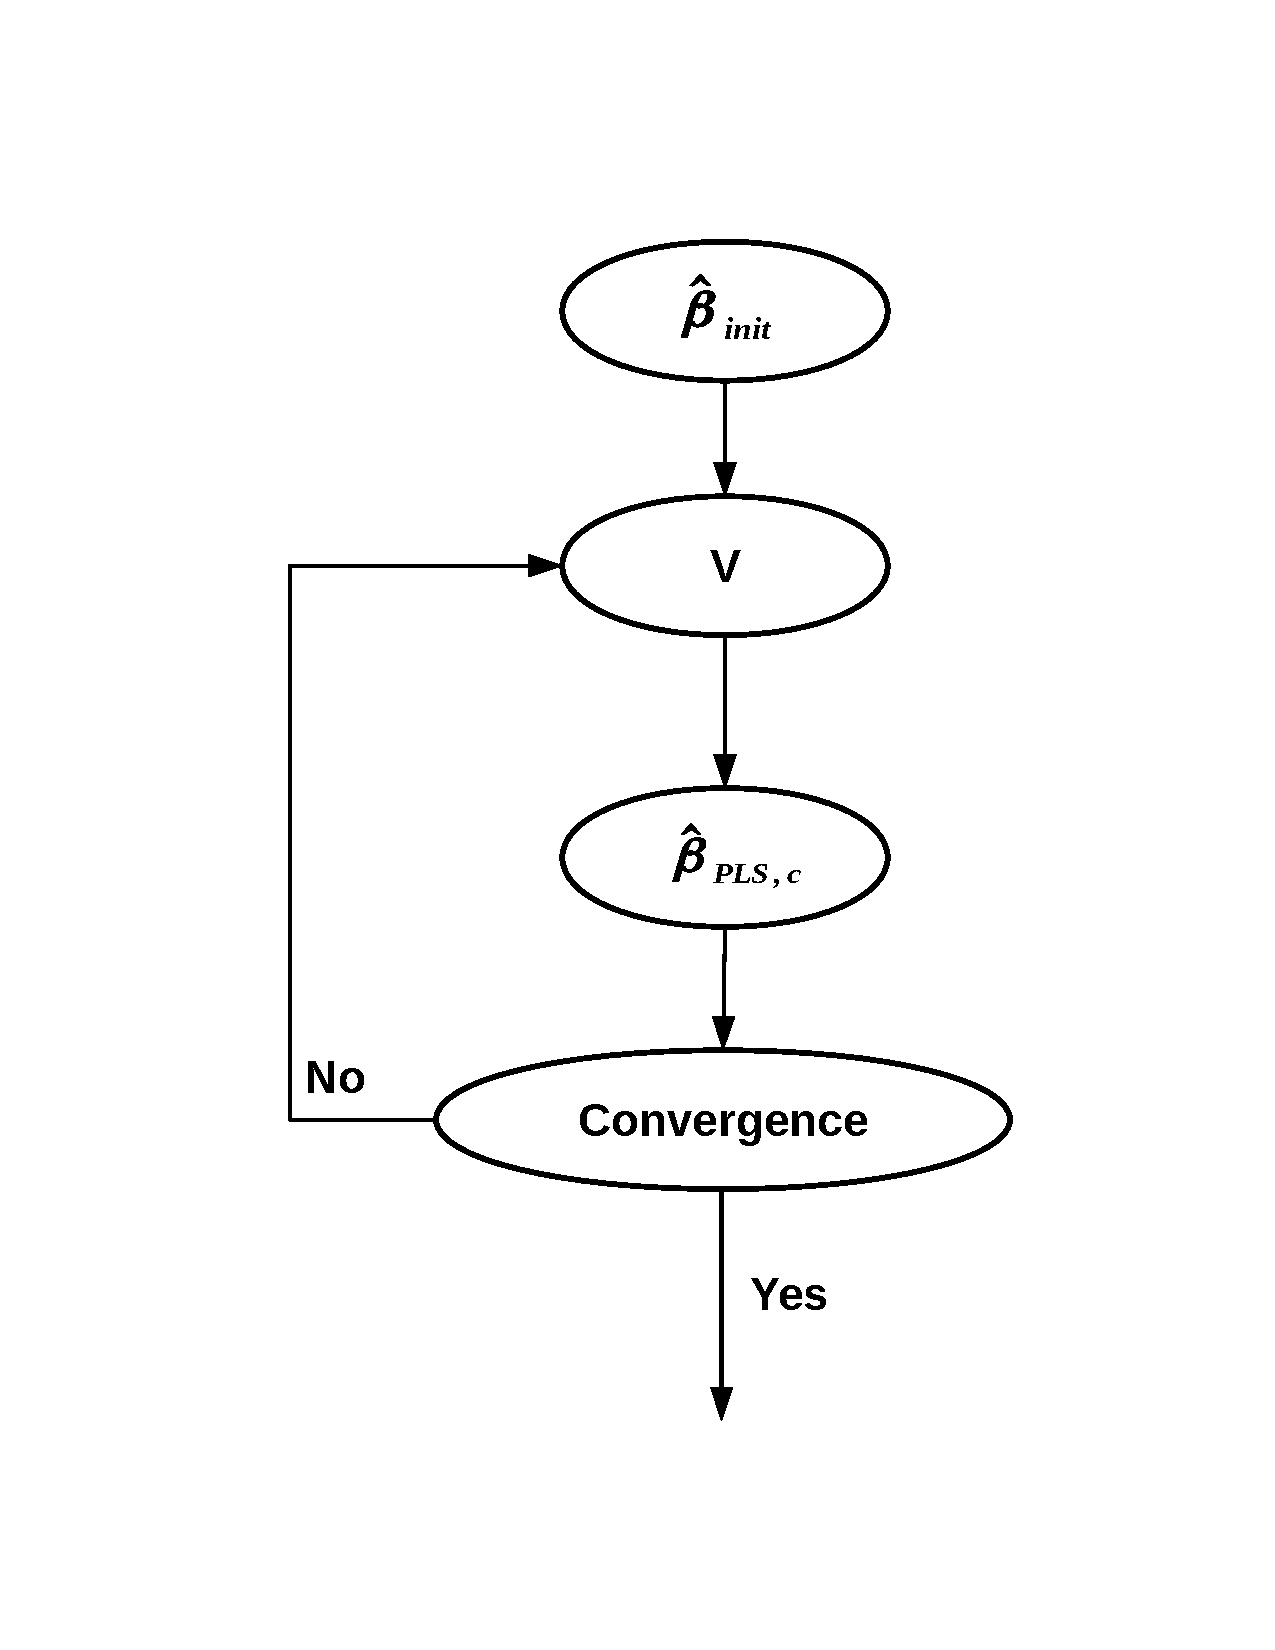
\includegraphics[width=0.6\linewidth]{../thesisplots/algorithm.pdf}
 		\caption{Penalized iteratively reweighted least squares algorithm}
 		\label{fig:pirls}
 	\end{figure}
 	  

	The initial estimate $\vec{\hat{\beta}}_{init}$ needed to compute the weighting matrix $\vec{V}$ is given by the least squares estimate $\vec{\hat{\beta}}_{LS}$. Now the calculation of the constrained least squares estimate $\vec{\hat{\beta}}_{PLS,c}$ and the calculation of the weighting matrix $\vec{V}$ is performed until no more changes in the weighting matrix $\vec{V}$ appear. This scheme is called penalized iteratively reweighted least squares and is abbreviated by PIRLS. \cite{hofner2011monotonicity}
	
	
	Figure \ref{fig:incspline} shows an example, where noisy data is approximated by considering the monotonicity constraint. The smoothing parameter was optimized using cross-validation, set to $\lambda_s=271.9$ and used for both estimates. The constraint parameter was set to $\lambda_c = 6000$. For both function estimations, the number of used splines $k$ was set to $30$. 	
	
	\begin{figure}[H]
		\centering
		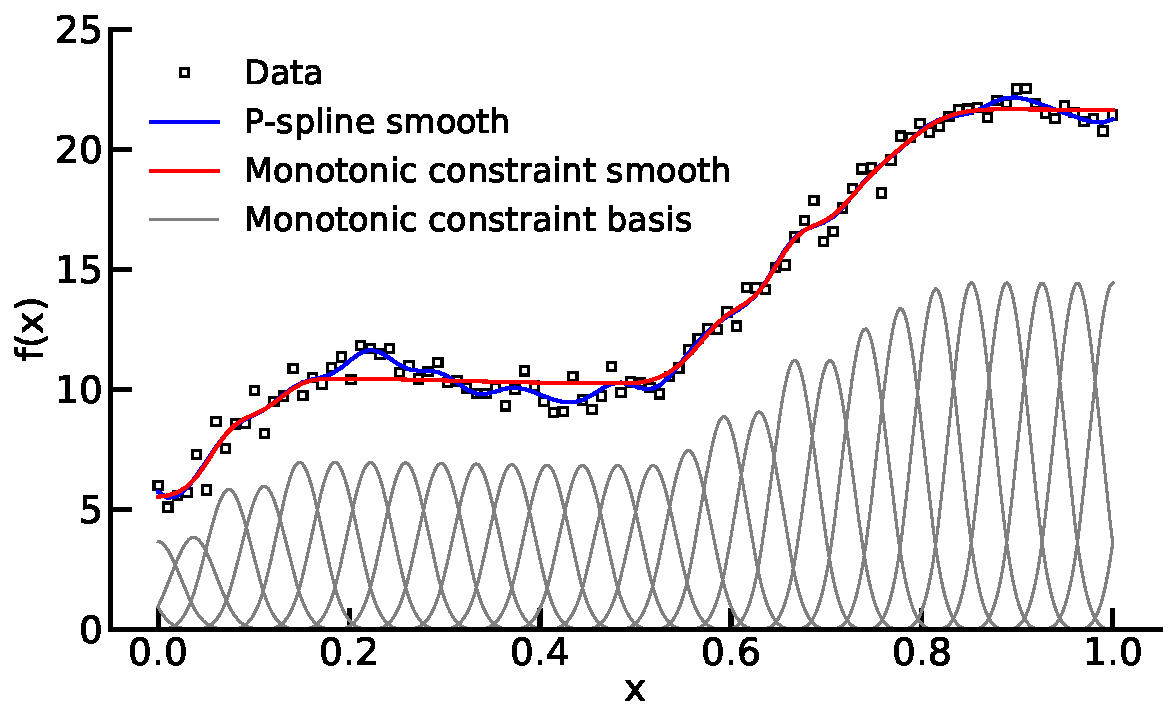
\includegraphics[width=\linewidth]{../thesisplots/inc_spline.pdf}
		\caption{Monotonic constrained 1d function estimation}
		\label{fig:incspline}
	\end{figure}	

	The red, constraint function estimation follows the monotonicity constraint far better that the blue, smooth function estimation. For $x \in [0, 0.2]$ and $x > 0.6$, the two fits are identical, since no constraint violation is present. The weighting matrix $\vec{V}$ is therefore $0$ everywhere and the constraint is not active. For $x \in [0.15, 0.6]$ the constraint is active. The red fit produces a almost constant line as optimal solution for the competing goals of data accuracy, smoothness and constraint fidelity.

	This shows, that the incorporation of a priori knowledge in the fitting process using B-splines is in principle possible using a appropriate choice of the mapping matrix $\vec{D}_c$ and the weighting matrix $\vec{V}$ as well as an iterative fitting approach using penalized iteratively reweighted least squares. 
		
	%%%%%%%%%%%%%%%%%%%%%%%%%%%%%%%%%%%%%%%%%%%%%%%%%%%%%%%%%%%%%%%%%%%%%%%%%%%%%%%%%%%%%%%%%%%%%%%%%%%%%%%%%%%%%%%%%
	%%%%%%%%%%%%%%%%%%%%%%%%%%%%%%%%%%%%%%%%%%%%%%%%%%%%%%%%%%%%%%%%%%%%%%%%%%%%%%%%%%%%%%%%%%%%%%%%%%%%%%%%%%%%%%%%%	
	\section{User-defined Constraints} \label{sec:user-defined-constraints}
	
	As stated before, a priori knowledge can be introduced by the choice of the mapping matrix $\vec{D}_c$ and the weighting matrix $\vec{V}$. It now follows a description of the different matrices, which are used to enforce a priori known behavior. 
	
	%%%%%%%%%%%%%%%%%%%%%%%%%%%%%%%%%%%%%%%%%%%%%%%%%%%%%%%%%%%%%%%%%%%%%%%%%%%%%%%%%%%%%%%%%%%%%%%%%%%%%%%%%%%%%%%%%
	\subsection{Monotonicity Constraint}
	
	The mapping matrix $\vec{D}_c^{monoton}$ enforcing monotonic behavior follows from the first order difference operator $\Delta^1$. The corresponding matrix for $k$ splines is given as
	
	\begin{align} \label{eq:D_c_monoton}
		\vec{D}_c^{monoton} = \begin{pmatrix}  -1 & 1  &  		& \\ 
		  												 & -1 & 1 		& \\ 
														 &    & \ddots  & \ddots  
		\end{pmatrix} \in \mathbb{R}^{k-1 \times k}.
	\end{align}
	The difference between monotonic increasing and decreasing behavior is controlled by the weighting matrix $\vec{V}$. For increasing behavior, the weighting matrix $\vec{V}$ is given by the weights $v_j$ according to
	
	\begin{align} \label{eq:v_monoton_inc}
		v_j(\vec{\beta}) = \begin{cases} 0, \quad \text{if} \ \Delta^1\beta_j \ge 0 \\ 
					        					1, \quad \text{if} \ \Delta^1\beta_j < 0.
			\end{cases}	
	\end{align}
	
	For decreasing behavior, the weighting matrix $\vec{V}$ is given by the weights $v_j$ according to
	\begin{align} \label{eq:v_monoton_dec}
		v_j(\vec{\beta}) = \begin{cases} 0, \quad \text{if} \ \Delta^1\beta_j \le 0 \\ 
						    					1, \quad \text{if} \ \Delta^1\beta_j > 0.
			\end{cases}	
	\end{align}
	This states, that the penalty term $\mathcal{J}_c(\vec{\beta}; c)$ only contributes if adjacent coefficients $\beta_{j-1}$ and $\beta_j$ are increasing or decreasing, respectively. \cite{hofner2011monotonicity} \cite{eilers2005unimodal}

	%%%%%%%%%%%%%%%%%%%%%%%%%%%%%%%%%%%%%%%%%%%%%%%%%%%%%%%%%%%%%%%%%%%%%%%%%%%%%%%%%%%%%%%%%%%%%%%%%%%%%%%%%%%%%%%%%	
	\subsection{Curvature Constraint}
	
	In the simplest case, the curvature of the function $f(x)$ can either be convex, i.e. $f''(x) \ge 0$, or concave, i.e. $f''(x) \le 0$. The mapping matrix $\vec{D}_c^{curvature}$ enforcing this behavior can be approximated by the second order difference operator $\Delta^2$. The corresponding matrix for $k$ splines is given as

	\begin{align} \label{eq:D_c_curvature}
		\vec{D}_c^{curvature} = \begin{pmatrix} 1 & -2 & 1 		&  		 & \\ 
														 & 1  &-2 	    &1 		 & \\
														 & 	  & \ddots  & \ddots & \ddots  
										\end{pmatrix} \in \mathbb{R}^{k-2 \times k}.
	\end{align}	
	
	The difference between concave and convex curvature is controlled by the weighting matrix $\vec{V}$. For concave behavior, the weighting matrix $\vec{V}$ is given by the weights $v_j$ according to
	
	\begin{align}\label{eq:v_curvature_concave}
		v_j(\vec{\beta}) = \begin{cases} 
										0, \quad \text{if} \ \Delta^2\beta_j \le 0 \\ 
										1, \quad \text{if} \ \Delta^2\beta_j > 0. 
								   \end{cases}
	\end{align}
	
	For convex curvature, the weighting matrix $\vec{V}$ is given by the weights $v_j$ according to

	\begin{align}\label{eq:v_curvature_convex}
		v_j(\vec{\beta}) = \begin{cases} 
										0, \quad \text{if} \ \Delta^2\beta_j \ge 0 \\ 
										1, \quad \text{if} \ \Delta^2\beta_j < 0. 
								  \end{cases}
	\end{align}	
	
	Therefore, the penalty term $\mathcal{J}_c(\vec{\beta}; c)$ only contributes if the second order difference of adjacent coefficients $\vec{\beta}$ is either positive or negative, respectively. \cite{eilers2005unimodal}
	
	%%%%%%%%%%%%%%%%%%%%%%%%%%%%%%%%%%%%%%%%%%%%%%%%%%%%%%%%%%%%%%%%%%%%%%%%%%%%%%%%%%%%%%%%%%%%%%%%%%%%%%%%%%%%%%%%%	
	\subsection{Unimodality Constraint}
	
	A function $f(x)$ is said to be unimodal if for some value $m$, it is monotonically increasing for $x \le m$ and monotonically decreasing for $x \ge m$. We assume that there is a peak in the data $\{x^{(i)}, y^{(i)}\}$ and therefore want to constrain the fit to include a peak.
	
	The mapping matrix $\vec{D}_c^{unimodal}$ enforcing unimodal behavior can be constructed using the first order difference operator $\Delta^1$. The weighting matrix $\vec{V}$ now has a special structure. 
	
	First, we construct the B-spline basis according to the given data. We then need to find the index $j_{peak}$ of the \emph{peak spline}, which has the maximal value at the peak data point, see Figure \ref{fig:peak_spline}. The index $j_{peak}$ is now used as splitting point for the weighting matrix $\vec{V}$. All coefficients $\beta_j$ for $j < j_{peak}$ are constrained to be monotonic increasing, i.e. $\Delta^1 \beta_j \ge 0$ for $j = 1, \dots, j_{peak}-1$, while all coefficients $\beta_j$ for $j > j_{peak}$ are constrained to be monotonic decreasing, i.e. $\Delta^1 \beta_j \le 0$ for $j = j_{peak}+1, \dots, k$. The coefficient $\beta_{j_{peak}}$ stays unconstrained. \cite{eilers2005unimodal} 
	
	\begin{figure}[H]
		\centering
		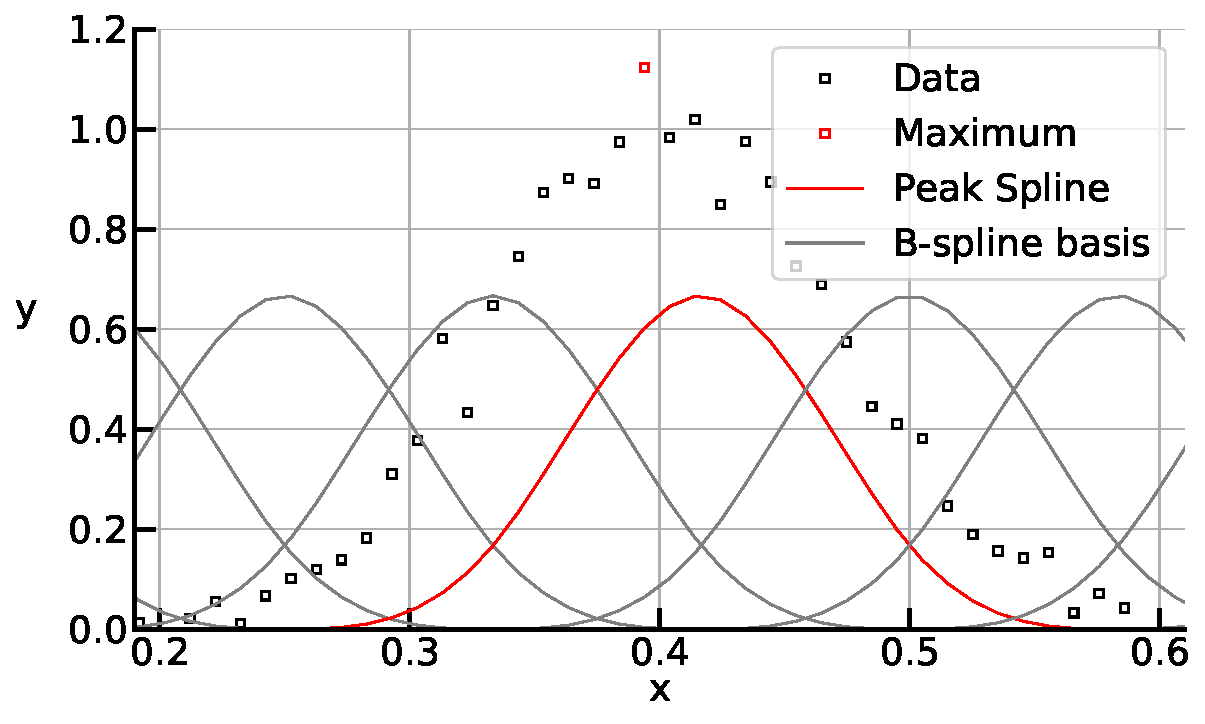
\includegraphics[width=\linewidth]{../thesisplots/peak_spline.pdf}
		\caption{Identification of the peak spline}
		\label{fig:peak_spline}
	\end{figure}
	
	
	The corresponding matrix for $k$ splines is given as 
	
	\begin{align}\label{eq:D_c_unimodal}
		\vec{D}_c^{unimodal} = \begin{pmatrix} -1 & 1 \\ 
									    				 & \ddots & \ddots  \\
									                     &        &     -1 & 1 & \\
									    			     & 		  & 	   & 0 & 0 & \\ 
													     &		  &		   &   &-1 & 1 \\
													     &		  &		   &   &   &\ddots & \ddots \\
													     & 	      &        &   &   &       &  -1    & 1
					 \end{pmatrix} \in \mathbb{R}^{k-1 \times k}
	\end{align}
	
	The weights $v_j$ to incorporate the peak constraint have the following structure:
	
	\begin{align}\label{eq:v_peak_1}
		v_j(\vec{\beta}) &= \begin{cases} 
										0, \quad \text{if} \ \Delta^1\beta_j \ge 0 \\ 
										1, \quad \text{if} \ \Delta^1\beta_j  < 0.
								  \end{cases}, \quad \text{if} \ j < j_{peak}
	\end{align}
	
	and 
	
	\begin{align}\label{eq:v_peak_2}
		v_j(\vec{\beta}) &= \begin{cases} 
								 		0, \quad \text{if} \ \Delta^1\beta_j \le 0 \\ 
								 		1, \quad \text{if} \ \Delta^1\beta_j > 0.
								  \end{cases}, \quad \text{if} \ j > j_{peak}
	\end{align}
	
	When assuming a valley in the data, the same approach as above can easily be used by multiplying the data with $-1$ or by always doing the inverse operation, i.e. finding the index $j_{valley}$ of the \emph{valley spline}, then constraining all splines for $j < j_{valley}$ to be monotonic decreasing, i.e. $\Delta^1 \beta_j \le 0$ for $j = 1, \dots, j_{valley}-1$, and all splines for $j > j_{valley}$ to be monotonic increasing, i.e. $\Delta^1 \beta_j \ge 0$ for $j = j_{valley}+1, \dots, k$. The coefficient $\beta_{j_{valley}}$ stays unconstrained. 
	
	The weights $v_j$ to consider a valley constraint are given by
	
	\begin{align}\label{eq:v_valley_1}
		v_j(\vec{\beta}) &= \begin{cases} 
										0, \quad \text{if} \ \Delta^1\beta_j \le 0 \\ 
										1, \quad \text{if} \ \Delta^1\beta_j > 0
								   \end{cases}, \quad \text{if} \ j < j_{valley}
	\end{align}
	
	and 
	
	\begin{align}\label{eq:v_valley_2}
		v_j(\vec{\beta}) &= \begin{cases} 
										0, \quad \text{if} \ \Delta^1\beta_j \ge 0 \\ 
										1, \quad \text{if} \ \Delta^1\beta_j < 0.
									\end{cases}, \quad \text{if} \ j > j_{valley}.
	\end{align}
	
	%%%%%%%%%%%%%%%%%%%%%%%%%%%%%%%%%%%%%%%%%%%%%%%%%%%%%%%%%%%%%%%%%%%%%%%%%%%%%%%%%%%%%%%%%%%%%%%%%%%%%%%%%%%%%%%%
	\subsection{Boundedness Constraint}
	
	For certain physical systems, it is known a priori that the measured quantity cannot be smaller than zero, i.e. $f(x) \ge 0$. Using data-driven modeling on noisy data can lead to predictions in the interpolation and extrapolation regime, which may not hold this constraint. It is therefore appropriate to apply the user-defined constraint of boundedness from below.
	
	The user-defined constraint for boundedness from below by $M=0$ uses a weighting matrix $\vec{V} \in \mathbb{R}^{n\times n}$, with individual weights $v_j$ specified as follows:
	
	\begin{align} \label{eq:v_boundedness}
		v_j(\vec{\beta}) = \begin{cases} 
										0, \quad \text{if} \ f(x^{(j)}) \ge M\\ 
										1, \quad \text{if} \ f(x^{(j)})  < M 		
			  \end{cases}
	\end{align}
	
	The constrained,penalized least squares objective function is then of the form
	
	\begin{align}\label{eq:OF_4}
		Q_4(\vec{y}, \vec{\beta}) = Q_1(\vec{y}, \vec{\beta}) + \lambda_s \mathcal J_s(\vec{\beta}; d) + \lambda_{bounded} \mathcal J_{bounded}(\vec{\beta}) 
	\end{align}
	
	where

	\begin{align}\label{eq:J_bounded}
	 	\mathcal J_{bounded} = \transpose{\vec{\beta}} \transpose{\vec{X}} \vec{V} \vec{X} \vec{\beta} 	
	\end{align}
	
	is the penalty term specifying boundedness from below by M and $\lambda_{bounded}$ is the constraint parameter, which is set multiple orders of magnitude higher than the smoothness parameter $\lambda_s$ to enforce the constraint. The matrix $\vec{X}$ is the B-spline basis. 
	
	Using different values of $M$ allows us to bound from below from any number $M$. Switching the comparison operators in (\ref{eq:v_boundedness}) enables us to bound functions from above. 
	
	%%%%%%%%%%%%%%%%%%%%%%%%%%%%%%%%%%%%%%%%%%%%%%%%%%%%%%%%%%%%%%%%%%%%%%%%%%%%%%%%%%%%%%%%%%%%%%%%%%%%%%%%%%%%%%%%
	\subsection{Jamming Constraint}
	
	Jamming the function $f(x)$ by some point $p = \{x^{(jamm)}, y^{(jamm)}\}$ means that the estimated function $f(x^{(jamm)}) \approx y^{(jamm)}$. This can be incorporated using the weighted least squares approach. \cite{strutz2016data} We can therefore use a priori knowledge that the estimated function should be in the proximity of $y^{(jamm)}$ for $x = x^{(jamm)}$. 
	
	The constraint, weighted objective function is then of the form
	
	\begin{align}\label{eq:OF_5}
		Q_5(\vec{y}, \vec{\beta}) = \lVert \vec{y} - \vec{X}\vec{\beta} \rVert^2_W
	\end{align}
	
	using the matrix norm $\lVert .\rVert_W$ induced by the weighting matrix $\vec{W} \in \mathbb{R}^{n \times n}$. The weights $w_i$ for $i=1, \dots, n$ are equal to $1$, except for the point $p$ for which the weight $w_p$ is set to some high value, e.g. $w_p = 1000$.
	
	By minimizing the objective function in (\ref{eq:OF_5}), i.e.
	
	\begin{align}\label{eq:optimization_problem_5}
		\vec{\hat \beta}_{WLS} = \arg \min_{\vec{\beta}} Q_5(\vec{y}, \vec{\beta}),
	\end{align}

	we obtain the weighted least squares estimate
	
	\begin{align} \label{eq:WLS_coef}
	\vec{\hat \beta}_{WLS} = (\transpose{\vec{X}} \vec{W} \vec{X})^{-1} \transpose{\vec{X}} \vec{W} \vec{y}.
	\end{align}	

	%%%%%%%%%%%%%%%%%%%%%%%%%%%%%%%%%%%%%%%%%%%%%%%%%%%%%%%%%%%%%%%%%%%%%%%%%%%%%%%%%%%%%%%%%%%%%%%%%%%%%%%%%%%%%%%%%
	%%%%%%%%%%%%%%%%%%%%%%%%%%%%%%%%%%%%%%%%%%%%%%%%%%%%%%%%%%%%%%%%%%%%%%%%%%%%%%%%%%%%%%%%%%%%%%%%%%%%%%%%%%%%%%%%%
	\section{n-d Constraint Function Estimation}
	
	The extension from one input to multiple input dimensions uses the concept of additive models given in Chapter \emph{Additive Models}. Given input data $\{ x_1^{(i)}, \dots, x_p^{(i)}, y^{(i)}\}$ for $i = 1, \dots, n$ and $p$ as the number of inputs, the combined model using all available B-splines and tensor-product splines is given as
	
	\begin{align} \label{eq:tps_all}
		y = f(x_1,..., x_p) = \sum_{j=1}^p s_j(x_j) + \sum_{j=1}^{p-1} \sum_{l>j}^p t_{j, l}(x_j, x_l)
	\end{align}
	
	where $s_j(x_j)$ is the B-spline estimate given by $s_j(x_j) = \vec{X}_j \vec{\beta}_j$ and $t_{l, j}(x_l,x_j)$ is the tensor-product estimate is given by $t_{j, l}(x_j,x_l) = \vec{X}_{j, l} \vec{\beta}_{j, l}$. The number of individual estimates is given by 
	
	\begin{align}
		n_{total} = p + \frac{p(p-1)}{2}.  
	\end{align}
	
	
	The constrained penalized least squares objective function for additive models can now be written similar to (\ref{eq:OF_3}) as
	
	\begin{align}\label{eq:OF_6}
		Q_6(\vec{y}, \vec{\beta}) = Q_1(\vec{y}, \vec{\beta}) + \transpose{\vec{\lambda}}_s	\vec{\mathcal{J}}_s(\vec{\beta}; \vec{d}) + \transpose{\vec{\lambda}}_c \vec{\mathcal{J}}_c(\vec{\beta}; \vec{c}).
	\end{align}
	
	with $\vec{\lambda}_s \in \mathbb{R}^{n_{total}}$ and  $\vec{\lambda}_c \in \mathbb{R}^{n_{total}}$  defined as vectors with one value of smoothness and constraint parameter for each estimate, respectively. 
	
	The objective function (\ref{eq:OF_6}) is then optimized, i.e.
	
	\begin{align}\label{eq:optimization_problem_6}
		\vec{\hat \beta}_{PLS,c,nd} = \arg \min_{\vec{\beta}} Q_5(\vec{y}, \vec{\beta}),
	\end{align}
	
	using the penalized iteratively reweighted least squares algorithm to obtain the coefficients $\vec{\hat{\beta}}_{PLS,c,nd}$. 
	
	We now need to specify the three parts of the objective function in (\ref{eq:OF_6}). 
	
	%%%%%%%%%%%%%%%%%%%%%%%%%%%%%%%%%%%%%%%%%%%%%%%%%%%%%%%%%%%%%%%%%%%%%%%%%%%%%%%%%%%%%%%%%%%%%%%%%%%%%%%%%%%%%%%%%
	\subsection{Data Term}
		

	
	Assuming the use of $k$ splines for the B-spline estimates and $k^2$ splines for the tensor-product estimates, the total number of coefficients to be determined is given by 
	
	\begin{align}\label{eq:tps_total_number_of_coef}
		k_{total} = pk + \frac{p(p-1)}{2}k^2. 
	\end{align}
	
	Since all B-spline and tensor-product spline models follow a linear model structure, we can combine them into one large model given by
	
	\begin{align}\label{eq:tps_lin_mod}
		\vec{y} = \vec{X} \vec{\beta}
	\end{align}
		
	where the matrix $\vec{X} \in \mathbb{R}^{n \times k_{total}}$ is given by a horizontal concatenation of the individual bases and the combined coefficient vector $\vec{\beta} \in \mathbb{R}^{k_{total}}$ is given by a vertical concatenation of the individual coefficient vectors. The model has then the following form
		
	\begin{align}\label{eq:tps_lin_model_verbose}
		\vec{y} = \vec{X} \vec{\beta} = 
					\begin{pmatrix} \vec{X}_{s_1} \dots \vec{X}_{s_p} \ \vec{X}_{t_{1,2}} \dots \vec{X}_{t_{p-1,p}} \end{pmatrix} 
					\begin{pmatrix} \vec{\beta}_{s_1} \\ 
									\vdots  \\ 
									\vec{\beta}_{s_p} \\ 
									\vec{\beta}_{t_{1,2}} \\ 
									\vdots \\ 
									\vec{\beta}_{t_{p-1,p}} \\
					\end{pmatrix}.
	\end{align}
	
	The data term $Q_1(\vec{y}, \vec{\beta})$ in the constrained penalized least squares objective function given in (\ref{eq:OF_6}) can now be evaluated using arbitrary input dimensions. 

	%%%%%%%%%%%%%%%%%%%%%%%%%%%%%%%%%%%%%%%%%%%%%%%%%%%%%%%%%%%%%%%%%%%%%%%%%%%%%%%%%%%%%%%%%%%%%%%%%%%%%%%%%%%%%%%%%
	\subsection{Smoothness Term}
	
	The combined smoothness penalty term $\vec{\mathcal{J}}_s(\vec{\beta}; \vec{d}) \in \mathbb{R}^{n_{total}}$ is then given as
	
	\begin{align}\label{eq:J_s_ndim}
		\vec{\mathcal{J}}_s(\vec{\beta}; \vec{d}) &= 
			\begin{pmatrix}
				\mathcal J_{s_1}(\vec{\beta}_{s_1}; d_{s_1}) \\ 
				\vdots \\ 
				\mathcal J_{s_p}(\vec{\beta}_{s_p}; d_{s_p}) \\
				\mathcal J_{t_{1,2}}(\vec{\beta}_{t_{1,2}}; d_{t_{1,2}}) \\
				\vdots \\
				\mathcal J_{t_{p-1,p}}(\vec{\beta}_{t_{p-1,p}}; d_{t_{p-1,p}}) \\
			\end{pmatrix}
	\end{align}
	
	with $\mathcal J_e(\vec{\beta}_e; d_e) = \transpose{\vec{\beta}}_e \transpose{\vec{D}}_{d_e} \vec{D}_{d_e} \vec{\beta}_e$ determining the smoothness penalty term using the coefficients $\vec{\beta}_e$ and mapping matrix $\vec{D}_{d_e}$ for each estimate $e$ for $e=s_1, \dots, s_p, t_{1,2}, \dots, t_{p-1,p}$. The vector $\vec{d} \in \mathbb{R}^{n_{total}}$ consists of the orders $d_e$ determining the mapping matrix $\vec{D}_{d_e}$ of the smoothness constraint for each individual estimate $e$. 

	%%%%%%%%%%%%%%%%%%%%%%%%%%%%%%%%%%%%%%%%%%%%%%%%%%%%%%%%%%%%%%%%%%%%%%%%%%%%%%%%%%%%%%%%%%%%%%%%%%%%%%%%%%%%%%%%%
	\subsection{Constraint Term}
	The combined constraint penalty term $\vec{\mathcal{J}}_c(\vec{\beta}; \vec{c}) \in \mathbb{R}^{n_{total}}$ is then given as
	
	\begin{align}\label{eq:J_c_ndim}
		\vec{\mathcal{J}}_c(\vec{\beta}; \vec{c}) &= 
		\begin{pmatrix}
		\mathcal J_{s_1}(\vec{\beta}_{s_1}; c_{s_1}) \\ 
		\vdots \\ 
		\mathcal J_{s_p}(\vec{\beta}_{s_p}; c_{s_p}) \\
		\mathcal J_{t_{1,2}}(\vec{\beta}_{t_{1,2}}; c_{t_{1,2}}) \\
		\vdots \\
		\mathcal J_{t_{p-1,p}}(\vec{\beta}_{t_{p-1,p}}; c_{t_{p-1,p}}) \\
		\end{pmatrix}
	\end{align}

	with $\mathcal J_e(\vec{\beta}_e; c_e) = \transpose{\vec{\beta}}_e \transpose{\vec{D}}_{c_e} \vec{V}_e \vec{D}_{c_e} \vec{\beta}_e$ determining the constraint penalty term using the coefficients $\vec{\beta}_e$, the mapping matrix $\vec{D}_{c_e}$ and the weighting matrix $\vec{V}_e$ for each estimate $e$ for $e=s_1, \dots, s_p, t_{1,2}, \dots, t_{p-1,p}$. The vector $\vec{c} \in \mathbb{R}^{n_{total}}$ consists of the constraint type $c_e$, e.g. monoton increasing, determining the mapping matrix $\vec{D}_{c_e}$ for each individual estimate $e$. 
	

	%%%%%%%%%%%%%%%%%%%%%%%%%%%%%%%%%%%%%%%%%%%%%%%%%%%%%%%%%%%%%%%%%%%%%%%%%%%%%%%%%%%%%%%%%%%%%%%%%%%%%%%%%%%%%%%%%%%%
	\subsection{Mapping Matrices for Tensor-Product Splines}
	
	The tensor-product spline basis is given by the Kronecker product of two B-spline bases, as depicted in Chapter \emph{Tensor-product splines}. To extend the framework of mapping matrices to two dimensions and tensor-product splines, we again use the concept of Kronecker products. 
	
	We want to penalize adjacent coefficient differences to enforce smoothness, but this time, in two dimensions. Therefore, an appropriate spatial neighbourhood needs to be defined. An example for such neighbourhood for the coefficient $\beta_{j, k}$ is given by the coefficients left and right, i.e. $\beta_{j-1, k}$ and $\beta_{j+1, k}$, and the coefficients above and below, i.e. $\beta_{j, k-1}$ and $\beta_{j,k+1}$. 
	
	Let us now define the mapping matrices $\vec{D}_{d_1}$ and $\vec{D}_{d_2}$ of orders $d_1$ and $d_2$ for each dimension, respectively. Using the Kronecker product, we generate the expanded mapping matrix $\vec{D}_{d_{1}, exp} = \vec{I}_{d_2} \otimes \vec{D}_{d_1}$ with the identity matrix $\vec{I}_{d_2} \in \mathbb{R}^{d_2 \times d_2}$ and $\vec{D}_{d_2,exp} = \vec{D}_{d_2} \otimes \vec{I}_{d_1}$ with the identity matrix $\vec{I}_{d_1} \in \mathbb{R}^{d_1 \times d_1}$. 
	
	Row-wise mappings of order $d_1$ and column-wise mappings of order $d_2$ are now obtained by applying the expanded difference matrix $\vec{D}_{d_1,exp}$ and $\vec{D}_{d_2,exp}$ to the coefficient vector $\vec{\beta}$, respectively. 
	
	Using these concepts, in principle every possible pair of one dimensional user-defined constraints can now be constructed, e.g. unimodality in two dimensions would be obtained using the unimodal penalty matrix depicted above for each dimension. 
	
	The penalty term for the constraint given by $c_1$ for dimension $1$ and $c_2$ for dimension $2$ then has the form
	
	\begin{align} \label{eq:J_c_tps}
		\mathcal J_c(\vec{\beta}; c_1, c_2) = \transpose{\vec{\beta}} \transpose{\vec{D}}_{c_1,exp} \vec{V}_1 \vec{D}_{c_1,exp} \vec{\beta} + \transpose{\vec{\beta}} \transpose{\vec{D}}_{c_2,exp} \vec{V}_2 \vec{D}_{c_2,exp} \vec{\beta}
	\end{align}
	
	with $\vec{D}_{c_1,exp} = \vec{I}_{d_2} \otimes \vec{D}_{c_1}$ and $\vec{D}_{c_2,exp} = \vec{D}_{c_2} \otimes \vec{I}_{d_1}$ as individual mapping matrices  and the weighting matrices $\vec{V}_1$ and $\vec{V}_2$ according to the given constraints.
		
	The constrained penalized least squares objective function in (\ref{eq:OF_6}) can now be used to estimate the coefficients $\vec{\beta}_{PLS,c, nd}$. \cite{fahrmeir2013regression}
	
	%%%%%%%%%%%%%%%%%%%%%%%%%%%%%%%%%%%%%%%%%%%%%%%%%%%%%%%%%%%%%%%%%%%%%%%%%%%%%%%%%%%%%%%%%%%%%%%%%%%%%%%%%%%%%%%%%%%
	\subsection{2-d Example}
	
	As example for the n-d constraint function estimation, we take a look at the function 
	
	\begin{align} \label{eq:2d_test_func}
		f(x_1, x_2) = 2\exp{\Big(-\frac{(x_1 - 0.25)^2}{0.08}\Big)} + x_2^2 + \eta
	\end{align}
	
	for $x_1 \in [0,1]$ and $x_2 \in [0,1]$ and random Gaussian noise $\eta$ with $\sigma_{noise} = 0.1$. Therefore we expect a peak in dimension $x_1$ as well as increasing behavior for dimension $x_2$, see Figure \ref{fig:2d_example}. The user-defined constraints are therefore $c_1 = \text{unimodal}$ and $c_2 = \text{monotonic increasing}$ Using this knowledge, we create a model with the following characteristics:
	
	\begin{itemize}
		\item B-spline smooth $s_1(x_1)$: $k_{x_1} = 50$, $c = c_1$, $\lambda_s = 1$ and $\lambda_c = 6000$
		\item B-spline smooth $s_2(x_2)$: $k_{x_2} = 50$, $c = c_2$, $\lambda_s = 1$ and $\lambda_c = 6000$
	\end{itemize}
		
	The fit for this model as well as the individual estimates $s_1(x_1)$ and $s_2(x_2)$ are shown in Figure \ref{fig:2d_example}. The model fits the data quite well and holds the specified constraints for the individual dimensions.
		
	\begin{figure}[H]
	\centering
	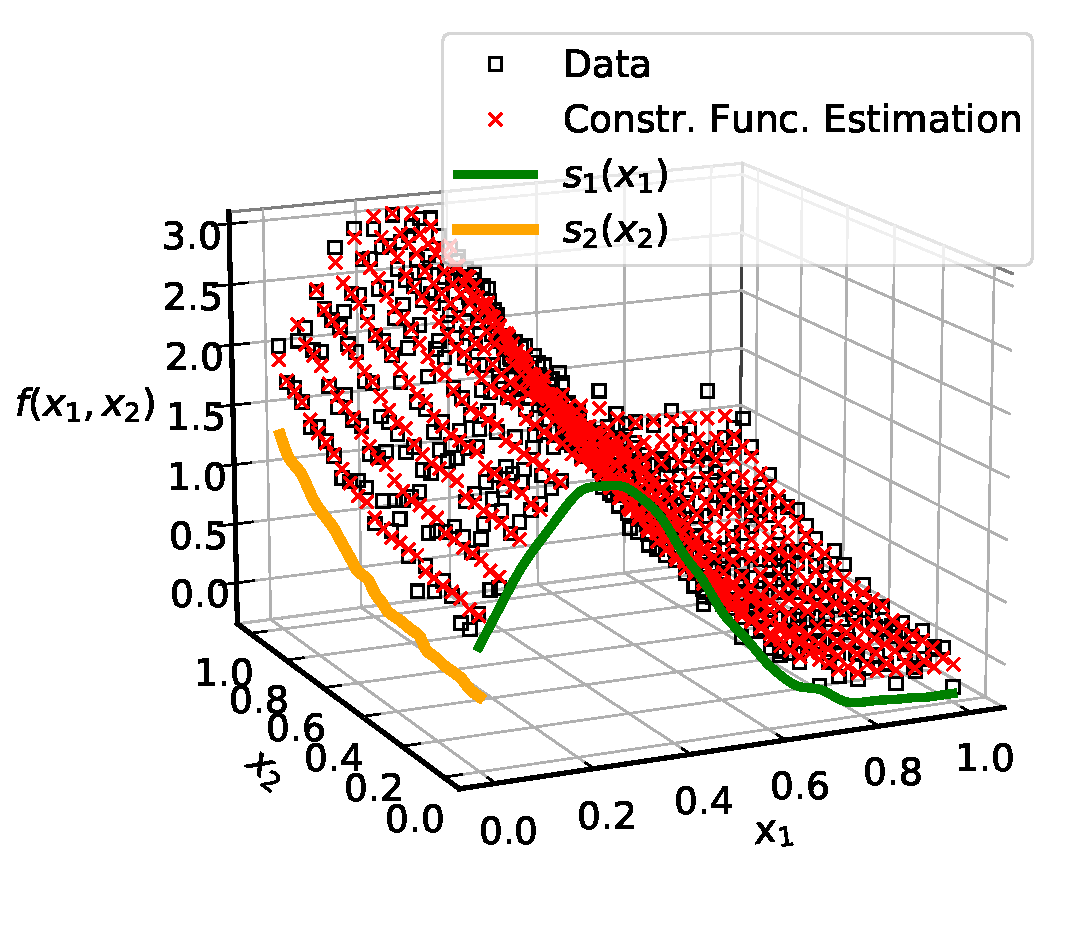
\includegraphics[width=\linewidth]{../thesisplots/2d_example.pdf}
	\caption{2-d test function for n-d constrained function estimation}
	\label{fig:2d_example}
	\end{figure}


	
\printbibliography
	
\end{document}